\documentclass[12pt, oneside]{article} 
\usepackage{amsmath, amsthm, amssymb, calrsfs, wasysym, verbatim, bbm, graphics, geometry, enumitem, array, multirow, hyperref, tabulary, mathtools, graphicx, tikz, listings, enumitem, bm, bbm}

\usepackage{amsfonts}
\usepackage[onehalfspacing]{setspace}

\usepackage{subcaption}


\setlength{\parindent}{0in} % set paragraph indent

\geometry{top=1in, bottom=1in, left=1in, right=1in}
\setlist{noitemsep}
%\setcounter{secnumdepth}{0} % comment this out for section numbering
\everymath{\displaystyle}


% Math symbols
\newcommand*{\T}{^{\top}}
\renewcommand*{\i}{\leftarrow}
\newcommand*{\isim}{\overset{\text{ind}}{\sim}}
\newcommand*{\iid}{\overset{\text{i.i.d.}}{\sim}}
\newcommand*{\deq}{\overset{\text{d}}{=}}
% Sets (natural numbers etc)
\newcommand*{\IN}{\mathbb{N}} 
\newcommand*{\IZ}{\mathbb{Z}}
\newcommand*{\IQ}{\mathbb{Q}}
\newcommand*{\IR}{\mathbb{R}}
\newcommand*{\IC}{\mathbb{C}}
% Distributions, processes
\newcommand*{\Geo}{\operatorname{Geo}}
\newcommand*{\Exp}{\operatorname{Exp}}
\newcommand*{\Poi}{\operatorname{Poi}}
\newcommand*{\NVM}{\operatorname{NVM}}
\newcommand*{\Par}{\operatorname{Par}}
\newcommand*{\IG}{\operatorname{IG}}
\newcommand*{\LN}{\operatorname{LN}}
\newcommand*{\Cauchy}{\operatorname{Cauchy}}
\newcommand*{\Log}{\operatorname{Log}}
\newcommand*{\U}{\operatorname{U}} % uniform distribution
\newcommand*{\B}{\operatorname{B}}
\newcommand*{\Bin}{\operatorname{Bin}}
\newcommand*{\Bern}{\operatorname{Bern}}
\newcommand*{\Beta}{\operatorname{Beta}}
\newcommand*{\NB}{\operatorname{NB}}
\newcommand*{\N}{\operatorname{N}}
% Operators, functions
\newcommand*{\I}{\mathbbm{1}} % indicator 
\newcommand*{\rd}{\mathrm{d}} % differential in integrals 
\renewcommand*{\mod}{\operatorname{mod}}
\newcommand*{\arginf}{\operatorname*{arginf}}
\newcommand*{\argsup}{\operatorname*{argsup}}
\newcommand*{\ran}{\operatorname{ran}}
\newcommand*{\rank}{\operatorname{rank}}
\newcommand*{\sign}{\operatorname{sign}}
\newcommand*{\round}{\operatorname{round}}
\renewcommand*{\L}{\mathcal{L}}
\renewcommand*{\Re}{\operatorname{Re}}
\renewcommand*{\Im}{\operatorname{Im}}
\newcommand*{\Li}{\operatorname*{Li}}
\renewcommand*{\P}{\mathbb{P}} % probability
\newcommand*{\E}{\mathbb{E}} % expected value 
\newcommand*{\med}{\operatorname{med}}
\newcommand*{\Var}{\operatorname{Var}}
\newcommand*{\Cov}{\operatorname{Cov}}
\newcommand*{\Cor}{\operatorname{Cor}}
\newcommand*{\MSE}{\operatorname{MSE}}
\newcommand*{\SE}{\operatorname{SE}}

% Variables
\newcommand*{\R}{\textsf{R}}
\newcommand*{\eps}{\varepsilon}
\renewcommand*{\th}{\bm{\theta}}
\newcommand*{\ba}{\bm{a}}
\newcommand*{\bnu}{\bm{\nu}}
\newcommand*{\bb}{\bm{b}}
\newcommand*{\be}{\bm{e}}
\newcommand*{\blambda}{\bm{\lambda}}
\newcommand*{\bzero}{\bm{0}}
\newcommand*{\bone}{\bm{1}}
\newcommand*{\bt}{\bm{t}}
\newcommand*{\bx}{\bm{x}}
\newcommand*{\by}{\bm{y}}
\newcommand*{\bz}{\bm{z}}
\newcommand*{\bu}{\bm{u}}
\newcommand*{\bU}{\bm{U}}
\newcommand*{\bv}{\bm{v}}
\newcommand*{\bw}{\bm{w}}
\newcommand*{\btheta}{\bm{\theta}}
\newcommand*{\bS}{\bm{S}}
\newcommand*{\bT}{\bm{T}}
\newcommand*{\bZ}{\bm{Z}}
\newcommand*{\bY}{\bm{Y}}
\newcommand*{\bX}{\bm{X}}
\newcommand*{\bmu}{\bm{\mu}}
% Estimators 
\newcommand*{\hgamma}{\widehat{\gamma}}
\newcommand*{\halpha}{\widehat{\alpha}}
\newcommand*{\hbeta}{\widehat{\beta}}
\newcommand*{\hlambda}{\widehat{\lambda}}
\newcommand*{\hmu}{\widehat{\mu}}
\newcommand*{\hp}{\widehat{p}}
\newcommand*{\hpi}{\widehat{\pi}}
\newcommand*{\hr}{\widehat{r}}
\newcommand*{\htau}{\widehat{\tau}}
\newcommand*{\htheta}{\widehat{\theta}}
\newcommand*{\hsigma}{\widehat{\sigma}}
\newcommand*{\tbeta}{\widetilde{\beta}}
\newcommand*{\tgamma}{\widetilde{\gamma}}
\newcommand*{\tlambda}{\widetilde{\lambda}}
\newcommand*{\tmu}{\widetilde{\mu}}
\newcommand*{\tpi}{\widetilde{\pi}}
\newcommand*{\tsigma}{\widetilde{\sigma}}
\newcommand*{\ttau}{\widetilde{\tau}}
\newcommand*{\barx}{\overline x}
\newcommand*{\barY}{\overline Y}
\newcommand*{\bary}{\overline y}
\newcommand*{\perm}[2]{{}^{#1}\!P_{#2}}%
\newcommand*{\comb}[2]{{}^{#1}C_{#2}}%
\usepackage{listings}
\lstset{ 
  language=R,               
  basicstyle=\small\ttfamily,   
  numbers=left,                  
  numberstyle=\tiny\color{gray},  
  stepnumber=1,                   
  showspaces=false,               
  showstringspaces=false,         
  showtabs=false,                  
  tabsize=4,                      
  captionpos=b,                   
  breaklines=true,               
  breakatwhitespace=false,        
  keywordstyle=\color{blue},    
  commentstyle=\color{purple}, 
  stringstyle=\color{Green}     
} 





\title{AFM 423}
\date{W2021}


\linespread{1.3}
\begin{document}

\maketitle

\newpage

\tableofcontents

\newpage

\section{Chapter 2:SL/ML}
\subsection{Splitting Data}
\begin{itemize}
    \item Training Set
    \item Test set: Not used during training
\end{itemize}

\subsection{Sampling}
\begin{itemize}
    \item \textbf{Simple random sample} (Ex: 70-30 split)
        \begin{verbatim}
        index <- sample(1:nrow(df), round(nrow(df) * 0.7))
        #caret package
        index <- createDataPartition(df$Sale_Price, p = 0.7, list = FALSE) 
        train_1 <- df[index, ]
        test_1 <- df[-index, ]
        \end{verbatim}
    \item \textbf{Stratified Sampling}: Training set and test set will have similar y distributions. Break y down into quantiles and randomly sample from each quantile. 
        \begin{verbatim}
        # stratified sampling with the rsample package
        split_strat <- initial_split(churn, prop = 0.7, strata = "Attrition")
        train_strat <- training(split_strat)
        test_strat <- testing(split_strat)
        \end{verbatim}
\end{itemize}


\subsection{Feature Engineering}
\begin{itemize}
    \item \textbf{One-hot encoding}: Transform categorical variables into numeric representations. Drop one level to create a full-rank (otherwise this results in perfect collinearity causing problems for some ML algorithms)
    
    \begin{verbatim}
    #full rank one-hot encode (caret package) - recommended for 
    #generalized linear models and neural networks
    full_rank <- dummyVars( ~ ., data = df, fullRank = TRUE)
    train_oh <- predict(full_rank, train_1)
    test_oh <- predict(full_rank, test_1)
    #less than full rank --> dummy encoding
    dummy <- dummyVars( ~ ., data = df, fullRank = FALSE)
    train_oh <- predict(dummy, train_1)
    test_oh <- predict(dummy, test_1)
    \end{verbatim}
    
    \item \textbf{Response Transformation}: Normalizing distribution of the response variable y (Get rid of skews).
    \begin{enumerate}
        \item Log transformation: normalize right skewed distributions
        \item Box Cox transformation $$g_\lambda(y) = \begin{cases}
            \frac{y^\lambda - 1}{\lambda} & ,\text{if } \lambda  \neq 0  \\ 
            log(y) &  ,\text{if } \lambda = 0 
        \end{cases}$$
        Where $\lambda$ is chosen by maximizing the log-likelihood function (RSS = residual sum of squares): $$L(\lambda) = -\frac{n}{2}\text{log}(\frac{RSS_\lambda}{n}) + (\lambda -1)\sum_{i=1}^{n}\text{log}(y_i)$$
    \end{enumerate}

    Note: Compute lambda on training set and use it for both training and test set to minimize data leakage
    
    \begin{lstlisting}
# Box Cox transformation
lambda <- forecast::BoxCox.lambda(train_1$Sale_Price)
train_bc_y <- forecast::BoxCox(train_1$Sale_Price, lambda)
test_bc_y <- forecast::BoxCox(test_1$Sale_Price, lambda)
    \end{lstlisting}
    
    Remember to re-transform the predicted values back to the original form
    
    \begin{lstlisting}
    # Inverse Box Cox function
    inv_box_cox <- function(x, lambda) {
     if (lambda == 0) exp(x) else (lambda*x + 1)^(1/lambda)
    }
    \end{lstlisting}
    
    \item \textbf{Predictor transformation}: some models require predictors to have the same units. 
    \begin{itemize}
        \item Centering and scaling can be used to standardize the predictors. (Gives 0 mean and unit variance)
        \item Normalizing predictor variables with Box Cox transformation.
        \item Collapsing highly correlated variables with PCA (reduces \# features and increases stability of generalized linear models) (Regularization is a better alternative to PCA since it doesn't reduce amount of information available).
        \item Removing near-zero/zero variance variables.
    \end{itemize} 

    Note: It is important to standardize test data based on the training mean and variance values of each predictor/feature
    
    \begin{verbatim}
    # identify only the predictor variables
    features <- setdiff(names(train_1), "Sale_Price")
    # pre-process estimation based on training features
    pre_process <- preProcess(
     x = train_1[, features],
     method = c("center", "scale")
     )
    pre_process_2 <- preProcess(
     x = train_1[, features],
     method = c("BoxCox", "center", "scale", "pca", "nzv")
     )
    # apply to both training & test
    train_x <- predict(pre_process, train_1[, features])
    test_x <- predict(pre_process, test_1[, features])    
    \end{verbatim}
\end{itemize}
 \newpage   
\subsection{Cross Validation for Generalization}
Goal: Find model that performs well on training data and \emph{future unseen data}
Take these models for example 
\begin{figure}[ht]
    \centering
     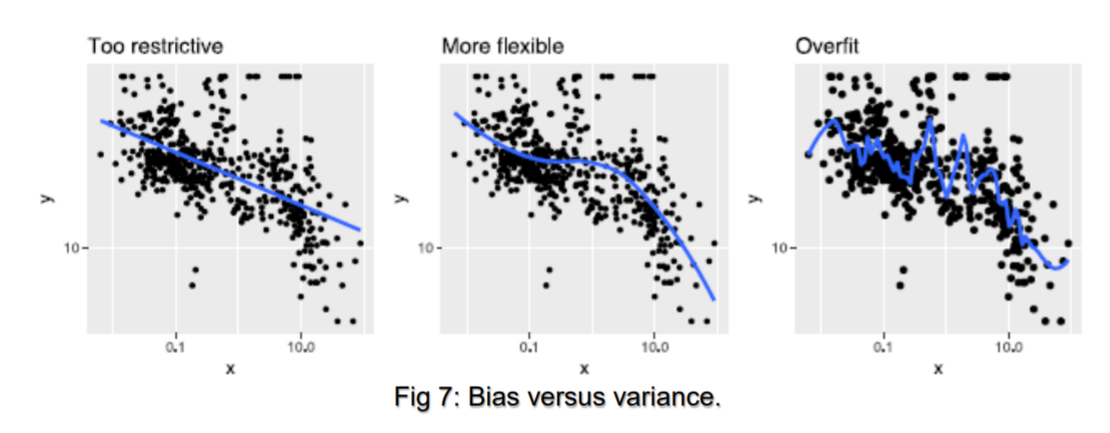
\includegraphics[width=1.0\textwidth]{Fig 7 Bias versus variance.png}
\end{figure}
\begin{itemize}
    \item \textbf{High bias}: Left model is too rigid/consistent and wouldn't change much for a new training sample. 
    \item \textbf{High Variance}: Right model 
\end{itemize}

To find a model that balances \emph{bias-variance trade-off}

\subsection{Model Evaluation}
Regression Models
\begin{itemize}
    \item MSE or RMSE: The squared component results in larger errors having larger penalties
    \begin{align*}
        MSE = \frac{1}{n}\sum_{i=1}^{n}(y_i - \widehat{y_i})^2
    \end{align*}
    \item Mean Residual:
    \begin{align*}
        MAE = \frac{1}{n}\sum_{i=1}^{n} |y_i - \widehat{y_i} |
    \end{align*}
    \item Mean Residual Deviance (Deviance): Provides \emph{goodness-of-fit} of the model when compared to the null model(intercept only). If response variable distribution then MRD = MSE. Otherwise, it gives a more useful estimate error.
    \item Root Mean Squared Logarithmic Error (RMSLE):
    \begin{align*}
        RMSLE = \sqrt{\frac{1}{n}\sum_{i=1}^{n}(log(y_i+1) - log(\widehat{y_i}+1))^2}
    \end{align*}
    \item R$^2$ = Proportion of variance in the response variable that is predictable from the predictors. \\
    \textbf{Limitation}: Two models from different data sets can have same RMSE but the one with less variability in the response variable would have a lower R$^2$. (Not the most important metric)
\end{itemize}
\subsection{Classification Models}
\begin{itemize}
    \item Misclassification Error: Total Misclassifications
    \item Mean per class error: Average classification errors per class
    \item Cross-entropy (Log Loss or Deviance): This metric disproportionately punishes predictions where we predict a small probability for the true class (Having high confidence in the wrong answer is really bad).
    \item Gini index: Measure of purity, a small value indicates that a node contains predominantly observations from a single class.
\end{itemize}

\subsubsection{Confusion Matrix}
Evaluate certain performance measures by counting true/false positives/negatives on categorical levels. Objective is to maximize the quantities below.
\begin{itemize}
    \item Accuracy: $\frac{TP + TN}{Total}$ \\
    \item Precision: $\frac{TP}{TP + FP}$ \\
    \item Sensitivity (recall): How accurately does the classifier classify actual events $\frac{TP}{TP + FN}$ \\
    \item Specificity: How accurately does the classifier classify actual non-events:
    $\frac{TN}{TN + FP}$ \\
    \item Area under the curve (AUC): A good classifier has \textbf{high precision + sensitivity} - minimizes FP and FN. AUC = area under ROC curve.
    \begin{itemize}
        \item Receiver Operating Characteristic (ROC) curve plots x = false positive rate, y = true positive rate. A y = x line represents a random guess. The higher the line the better performance of the model. 
    \end{itemize}
\end{itemize}
\begin{figure}[ht]
    \centering
     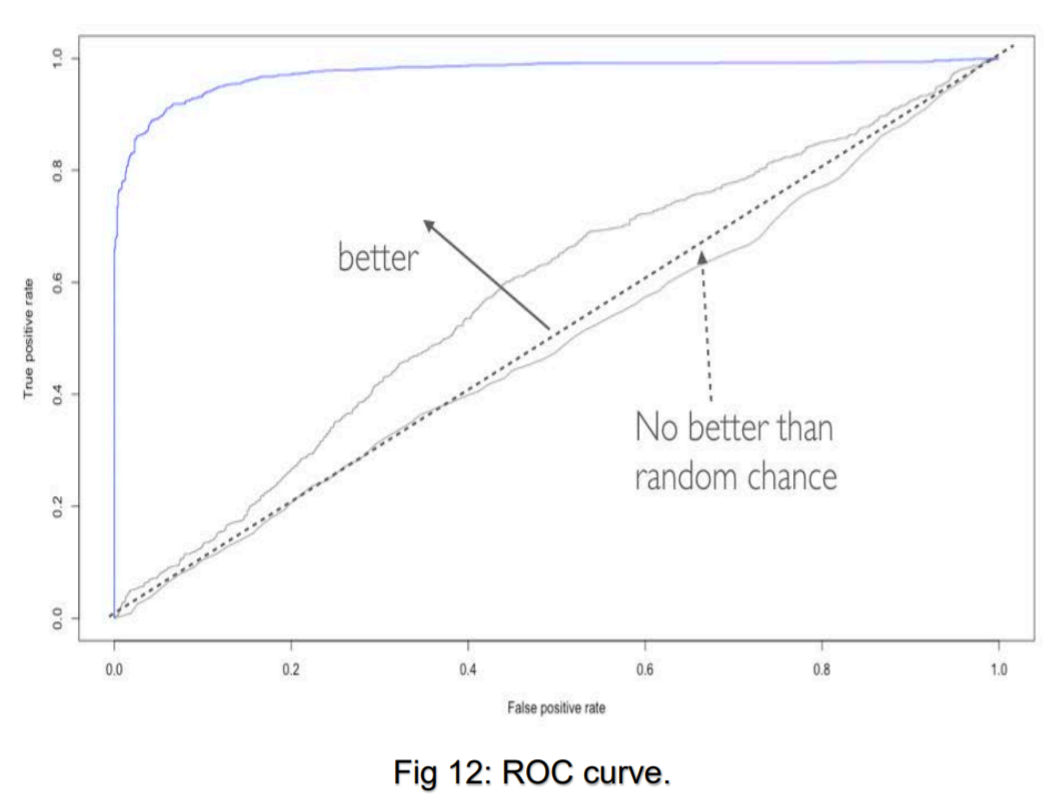
\includegraphics[width=1.0\textwidth]{ROC curve.png}
\end{figure}

\section{Linear Regression}

\subsection{Replication Requirements}
 \begin{lstlisting}
 ## Packages
library(tidyverse) # data manipulation and visualization
library(modelr) # provides easy pipeline modeling functions
library(broom) # helps to tidy up model outputs
tidy(model1)
## term estimate std.error statistic p.value
## 1 (Intercept) 6.76409784 0.6075916 11.13264 3.307215e-20
## 2 TV 0.05028368 0.0034632 14.51943 3.413075e-28
 \end{lstlisting}

\subsection{Standard Error}
\begin{align*}
    [\widehat{SE}(\hat{\beta_0})]^2 &= \hat{\sigma}^2 \left[\frac{1}{n} + \frac{\barx}{\sum^n_{i=1} (x_i - \barx)^2} \right]\\
    [\widehat{SE}(\hat{\beta_1})]^2 &= \frac{\hat{\sigma}^2}{\sum^n_{i=1} (x_i - \barx)^2} \\
    \hat{\sigma^2} &= \widehat{Var}(\hat{\epsilon_i}
 \end{align*}
 
 95\% Confidence intervals for each coefficient estimates:
 
 \begin{align*}
     \hat{\beta_0} &= \pm 1.96 \times  \widehat{SE}(\hat{\beta_0}) \\
     \hat{\beta_1} &= \pm 1.96 \times  \widehat{SE}(\hat{\beta_1})
 \end{align*}

\begin{lstlisting}
 ## confint(model1)
\end{lstlisting}

\subsection{T-statistic and p-value}
\begin{itemize}
    \item T-statistic measures the number of estimated standard deviations that $\beta_i$ is away from 0.
    \item Large t-statistic = small p-value.
    \begin{align*}
        t_0 =  \frac{\hat{\beta_i} - 0}{\widehat{SE}(\beta_i)}
    \end{align*}
    \item p-value = how likely that we will observe such a substantial association between the predictor and the response due to chance. 
    \item $H_0$: $\beta_i$ = 0 \\
    $H_a$: $\beta_i \neq 0$\\
    A small p-value means that the sample result would be unlikely if the null hypothesis were true. If there is less than 5\% chance of a result as extreme as the sample result if the null hypothesis were true (p-value), then the null hypothesis is rejected.
\end{itemize}

\subsection{Assessing Model Accuracy}
\begin{itemize}
   \item Residual Standard Error (RSE): An estimate of the standard deviation $\hat{\epsilon}$. It is the average amount that the response will deviate from the true regression line. 
   \begin{align*}
       RSE = \sqrt{\frac{1}{n-2}\sum^n_{i=1}(y_i-\widehat{y_i})^2}
   \end{align*}
   For an unbiased estimator we have 
   \begin{align*}
       bias(\hat{\theta)} =E(\theta) - \theta = 0 
   \end{align*}
   Note: An unbiased estimator is not always the better estimator
   \item R$^2$
   $$R^2 = 1- \frac{RSS}{TSS} = 1 - \frac{\sum^n_{i=1}(y_i-\widehat{y_i})^2}{\sum^n_{i=1}(y_i-\overline{y})^2}$$ \\ \\
   In the SLR model, the $R^2$ value is equal to the squared correlation between X and Y:
   \begin{lstlisting}
rsquare(model1, data = train)
cor(train$TV, train$Sales)^2
   \end{lstlisting}
  
   \item F-statistic: Test whether at least one predictor has a non-zero coefficient
   \begin{align*}
       F = \frac{(TSS-RSS)/p}{RSS/(n - p - 1)}
   \end{align*}
   where p is the number of parameters. Larger F-statistic = small p-value
   
\end{itemize}

\subsection{Multiple Linear Regression}
\begin{itemize}
    \item F-statistic $\approx$ 1 if there is no relationship between the response and predictors.
    \item F-statistic $> 1$  if otherwise
\end{itemize}

\subsection{Incorporating Interactions}

\section{k-NN for Regression}
\subsection{Parametric versus Non-Parametric Regression Models}
\begin{itemize}
    \item Suppose that we observe $Y-i$ and $X_i = (X_i1, ...,X_ip)$ for i = 1,...,n
    \item We can model the relationship as 
    \begin{align*}
        Y_i = f(X_i) + \epsilon_i
    \end{align*}
    where f is an unknown function and $\epsilon_i$ is a random error with mean 0. 
    \item Ideal f(X) or regression function: f(x) = E(Y$|$X=x)
    \item Parametric Estimate: Assume specific function form for the regression function: I.e. Assume linear functional form
    \begin{align*}
        f(x) = \beta_0  + \beta_1x_1 + ... + \beta_px_p
    \end{align*}
    \item Non-parametric approach considers \emph{locality}:
    \begin{align*}
         \widehat{f}(x) = \text{average}({y_i:x_i=x})
    \end{align*}
    as often no points will satisfy the requirement that:
    \begin{align*}
         \widehat{f}(x) = \text{average}({y_i:x_i=\text{(or very close to)}x})
    \end{align*}
    \item How do we figure out what is local? What is "close to" being local?
    \begin{enumerate}
        \item Neighbors (knn)
        \item Neighborhoods (Trees)
    \end{enumerate}
\end{itemize}

\subsection{k-Nearest Neighbors}
\begin{align*}
    \hat{f_k}(x) = \frac{1}{k}\sum_{i\in N_k(x,D)}y_i
\end{align*}
\begin{itemize}
    \item Nearest is usually defined by Euclidean Distance
    \item k-NN involves an implicit minimization(compared to explicit minimization in lm()).
    \item With k-NN, fitting amounts to picking a k, and seeing the training data.
    \item For a linear regression function: lm() performs well while knn "automatically" approximates the regression function.
    \item For a high non-linear regression function, lm() performs badly, while knn "automatically approximates the regression function.
\end{itemize}
\subsection{Scaling Data}
\begin{itemize}
    \item 
\end{itemize}
\end{document}